\documentclass[aspectratio=169]{beamer}
\usepackage{pgfpages}

\usepackage{datetime}
\newdateformat{mydate}{\THEYEAR-\twodigit{\THEMONTH}-\twodigit{\THEDAY}}

\usepackage[backend=biber, style=ieee]{biblatex}
\addbibresource{Bibliography.bib}
\renewcommand{\bibfont}{\tiny}

\usepackage{subcaption}
\usepackage{graphicx}
\usepackage{multicol}
\usepackage{algorithm}
\usepackage{algorithmic}
\usepackage{animate}
\usepackage{appendixnumberbeamer}
\usepackage{etoolbox}
\usepackage{adjustbox}
\usepackage{multimedia}


\usepackage[font=footnotesize]{caption}
\usepackage{color, colortbl}
\usepackage{multirow}

% \usepackage[acronym]{glossaries}
% \makenoidxglossaries
% \input{acronym.tex}

\usetheme{Warsaw}
\setbeamertemplate{navigation symbols}{}

\setbeamertemplate{bibliography item}{\insertbiblabel}
\setbeamertemplate{blocks}[rounded][shadow=false]

\makeatletter
\pgfdeclareverticalshading[lower.bg,upper.bg]{bmb@transition}{200cm}{%
  color(0pt)=(lower.bg); color(2pt)=(lower.bg)
}
\makeatother

\setbeamertemplate{blocks}[rounded][shadow=false]

\definecolor{unibe_white}{RGB}{243,252,240} % #f3fcf0
\definecolor{unibe_black}{RGB}{19, 17, 16} % #131110
\definecolor{unibe_prim}{RGB}{226, 0, 43} % #e2002b
\definecolor{unibe_bis}{RGB}{234, 144, 16} % #ea9010
\definecolor{unibe_ter}{RGB}{255, 210, 63} % #ffd23f

% \definecolor{unibe_prim_high}{RGB}{255, 235, 238}
% \definecolor{unibe_prim_low}{RGB}{102, 0, 19}

\setbeamertemplate{frametitle}[default]

\setbeamercolor{normal text}{fg=unibe_white}
\usebeamercolor[fg]{normal text}
\usebeamercolor[bg]{normal text}

\setbeamercolor{background canvas}{bg=unibe_black}

\setbeamercolor{structure}{fg=unibe_white}
\setbeamercolor{frametitle}{bg=unibe_black, fg=unibe_white}
\setbeamercolor{frametitle right}{bg=unibe_black, fg=unibe_white}
% \setbeamercolor{footlinecolor}{fg=unibe_black,bg=unibe_white}

\setbeamertemplate{itemize item}{\scalebox{0.45}{$\blacksquare$}}
\setbeamertemplate{itemize subitem}{{$\circ$}}
\setbeamertemplate{enumerate item}{\roman{enumi}}

\newenvironment<>{box_default}[1]{%
  \setbeamercolor{block title}{use=unibe_white,fg=unibe_black,bg=unibe_white}%
  \setbeamercolor{block body}{bg=unibe_black}
  \setbeamercolor{itemize item}{fg=unibe_white}
  \setbeamercolor{itemize subitem}{fg=unibe_white}
  \begin{block}#2{\centering \textbf{#1}}}{\end{block}}

% \newenvironment<>{box_col_prim}[1]{%
%   \setbeamertemplate{block title}[shadow=false]
%   \setbeamercolor{block title}{use=unibe_prim,fg=unibe_white,bg=unibe_prim}
%   \setbeamercolor{block body}{bg=unibe_prim_high, fg=unibe_prim_low}
%   \setbeamercolor{itemize item}{fg=unibe_prim_low}
%   \setbeamercolor{itemize subitem}{fg=unibe_prim_low}
%   \begin{block}#2{\centering \textbf{#1}}}{\end{block}}

\newenvironment<>{box_prim}[1]{%
  \setbeamercolor{block title}{use=unibe_prim,fg=unibe_white,bg=unibe_prim}%
  \setbeamercolor{block body}{bg=unibe_black}
  \setbeamercolor{itemize item}{fg=unibe_prim}
  \setbeamercolor{itemize subitem}{fg=unibe_prim}
  \begin{block}#2{\centering \textbf{#1}}}{\end{block}}

\newenvironment<>{box_bis}[1]{%
  \setbeamercolor{block title}{use=unibe_bis,fg=unibe_white,bg=unibe_bis}%
  \setbeamercolor{block body}{bg=unibe_black}
  \setbeamercolor{itemize item}{fg=unibe_bis}
  \setbeamercolor{itemize subitem}{fg=unibe_bis}
  \begin{block}#2{\centering \textbf{#1}}}{\end{block}}

\newenvironment<>{box_ter}[1]{%
  \setbeamercolor{block title}{use=unibe_ter,fg=unibe_black,bg=unibe_ter}%
  \setbeamercolor{block body}{bg=unibe_black}
  \setbeamercolor{itemize item}{fg=unibe_ter}
  \setbeamercolor{itemize subitem}{fg=unibe_ter}
  \begin{block}#2{\centering \textbf{#1}}}{\end{block}}

\newcommand{\textprim}[1]{\textcolor{unibe_prim}{#1}}
\newcommand{\textbis}[1]{\textcolor{unibe_bis}{#1}}
\newcommand{\textter}[1]{\textcolor{unibe_ter}{#1}}


% For a title slide to each section
% \AtBeginSection[]{
%   \begin{nonumberframe}{Table of contents}{\insertsection}
%     \centering
%     \tableofcontents[currentsection,hideothersubsections]
%   \end{nonumberframe}
% }

\setbeamertemplate{section in toc}[circle]
\setbeamertemplate{subsection in toc}[square]

\setbeamerfont{section number projected}{size=\large}
\setbeamercolor{section number projected}{fg=unibe_black,bg=unibe_white}

% \AtBeginSubsection[]{
%   \begin{nonumberframe}
%   \vfill
%   \centering
%   \begin{beamercolorbox}[sep=8pt,center,shadow=true,rounded=true]{title}
%     \usebeamerfont{title}\insertsubsectionhead\par%
%   \end{beamercolorbox}
%   \vfill
%   \end{nonumberframe}
% }

\usepackage[footheight=1em]{beamerthemeboxes}

\newenvironment{nonumberframe}{%
    \setbeamertemplate{footline}{%
    \leavevmode%
    \hbox{\begin{beamercolorbox}[wd=.99\paperwidth,leftskip=.3cm,rightskip=.3cm]{footlinecolor}%
    \insertsubtitle ~- \insertshortauthor
    \end{beamercolorbox}%
    }%
    \vskip 0pt%
    }
    \begin{frame}[noframenumbering] %Remove the noframenumbering option if you want the counter to be increased on a frame that is not numbered.
    }{%
    \end{frame}
}

\makeatother
\setbeamertemplate{footline}
{%
  \leavevmode%
  \hbox{\begin{beamercolorbox}[wd=.8\paperwidth,leftskip=.3cm,rightskip=.3cm]{footlinecolor}%
  \insertsubtitle ~- \insertshortauthor
  \end{beamercolorbox}%
  \begin{beamercolorbox}[wd=.19\paperwidth,leftskip=.3cm,rightskip=.3cm]{footlinecolor}%
    \hfill\insertframenumber/\inserttotalframenumber
  \end{beamercolorbox}
  }%
  \vskip 0
}
\makeatletter

\title{LIF and Simplified SRM Neurons Encode Signals Into Spikes \\ via a Form of Asynchronous Pulse Sigma-Delta Modulation \\ Young C. Yoon \cite{yoon_lif_2017}}
\subtitle{GUT meeting 2026-11-10}
\author[X. Lesage]{Xavier Lesage\\
Review: Luke Eilers}
\institute{NeuroTMA, Department of Physiology, University of Bern}
\date{\today}

\begin{document}

\begin{nonumberframe}
  % \begin{beamercolorbox}[sep=8pt,center,rounded=true]{title}
    \centering
    \usebeamerfont{title}\inserttitle\par%
    \usebeamerfont{subtitle}\insertsubtitle
  % \end{beamercolorbox}%

  \vspace{0.3cm}

  \begin{columns}[c]
    \begin{column}{0.35\paperwidth}
      \begin{figure}
        \centering
        
\includegraphics[width=.35\columnwidth]{Logos/Logo_NeuroTMA_final_white_transparent.png}
    \end{figure}
      \vspace{-0.5cm}
    \begin{figure}
        \centering
        \includegraphics[width=.5\columnwidth]{Logos/Unibe_white-transparent_logo.png}
    \end{figure}
    \end{column}

    \begin{column}{0.64\paperwidth}
      \usebeamerfont{author}\insertauthor\par
      \vspace{0.3cm}
      \usebeamerfont{institute}\insertinstitute\par
      \usebeamerfont{date}\insertdate
    \end{column}
  \end{columns}
\end{nonumberframe}

\section{Motivation}
\begin{frame}{Why spikes ?}{\insertsection}
    \begin{itemize}
        \item An approach from \textprim{Analog-to-Digital conversion} and \textprim{digital communications}
        \item Spiking mechanism as a conversion from analog ( continuous time, continuous space) to digital (discrete time and/or discrete space)
        \item How can we exploit this mechanism to design digital hardware ?
    \end{itemize}
    \begin{figure}
        \centering
        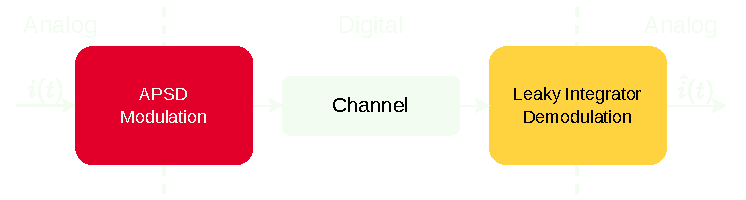
\includegraphics[width=.8\columnwidth]{Figures/overview.pdf}
    \end{figure}
\end{frame}

\section{Spike Response Model}
\subsection{Neuron Model}
\begin{frame}{Spike Response Model $0^{th}$ order \cite{gerstner_spiking_2002}}{\insertsection ~- \insertsubsection}
    \begin{columns}
        \column{0.35\paperwidth}
        \begin{figure}
            \centering
            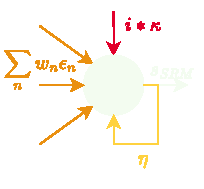
\includegraphics[width=.8\columnwidth]{Figures/srm_neuron.pdf}
        \end{figure}
        \vspace{-0.7cm}
        \begin{itemize}
            \item $\kappa$ : input response
            \item $\eta$ : output response
            \item $\epsilon$ : presynaptic spike response
        \end{itemize}

        \column{0.6\paperwidth}
        \begin{align*}
            v_{SRM}(t) = \textprim{i(t) * \kappa (t)} &+ \\
            \textter{\sum_{m=1}^{M_{SRM}} \eta(t-T_m^{SRM})} &+ \\
            \textbis{\sum_{n=1}^{N} w_n \sum_{m_n=1}^{M_n} \epsilon_n (t-T^{n}_{m_n})}\\
            s_{SRM}(t) \triangleq \sum_{m=1}^{M_{SRM}} \delta (t-T_m^{SRM})
        \end{align*}
    \end{columns}
\end{frame}

\begin{frame}{Alternative Form}{\insertsection ~- \insertsubsection}
    \begin{columns}
    \column{0.45\paperwidth}
    \begin{align*}
        y_{SRM}(t) &\triangleq i(t) * \kappa (t)\\
        \hat{y}_{SRM,L}(t) &\triangleq - \sum_{m=1}^{M_{SRM}} \eta(t-T_m^{SRM})\\
        &= -\eta(t) * s_{SRM}(t)\\
        v_{SRM}(t) &= y_{SRM}(t) - \hat{y}_{SRM,L}(t)
    \end{align*}

    \column{0.5\paperwidth}
    \begin{itemize}
        \item $y_{SRM}(t)$ : input current response filter
        \item $\hat{y}_{SRM,L}(t)$ : unsmoothed reconstruction estimate of $y_{SRM}(t)$
    \end{itemize}

    \begin{box_prim}{Remark}
        \begin{itemize}
            \item Tracking error is bounded by $v_t$
        \end{itemize}
    \end{box_prim}

    \end{columns}
\end{frame}

\begin{frame}{Filter Building Block}{\insertsection ~- \insertsubsection}
    \begin{figure}
        \centering
        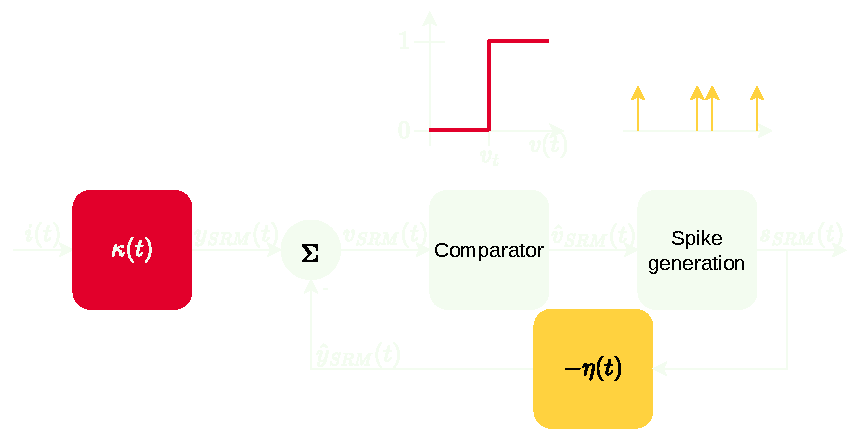
\includegraphics[width=.9\columnwidth]{Figures/srm_filter.pdf}
    \end{figure}
\end{frame}

\begin{frame}{Signals}{\insertsection ~- \insertsubsection}
    \begin{columns}
    \column{0.45\paperwidth}
    \begin{figure}
        \centering
        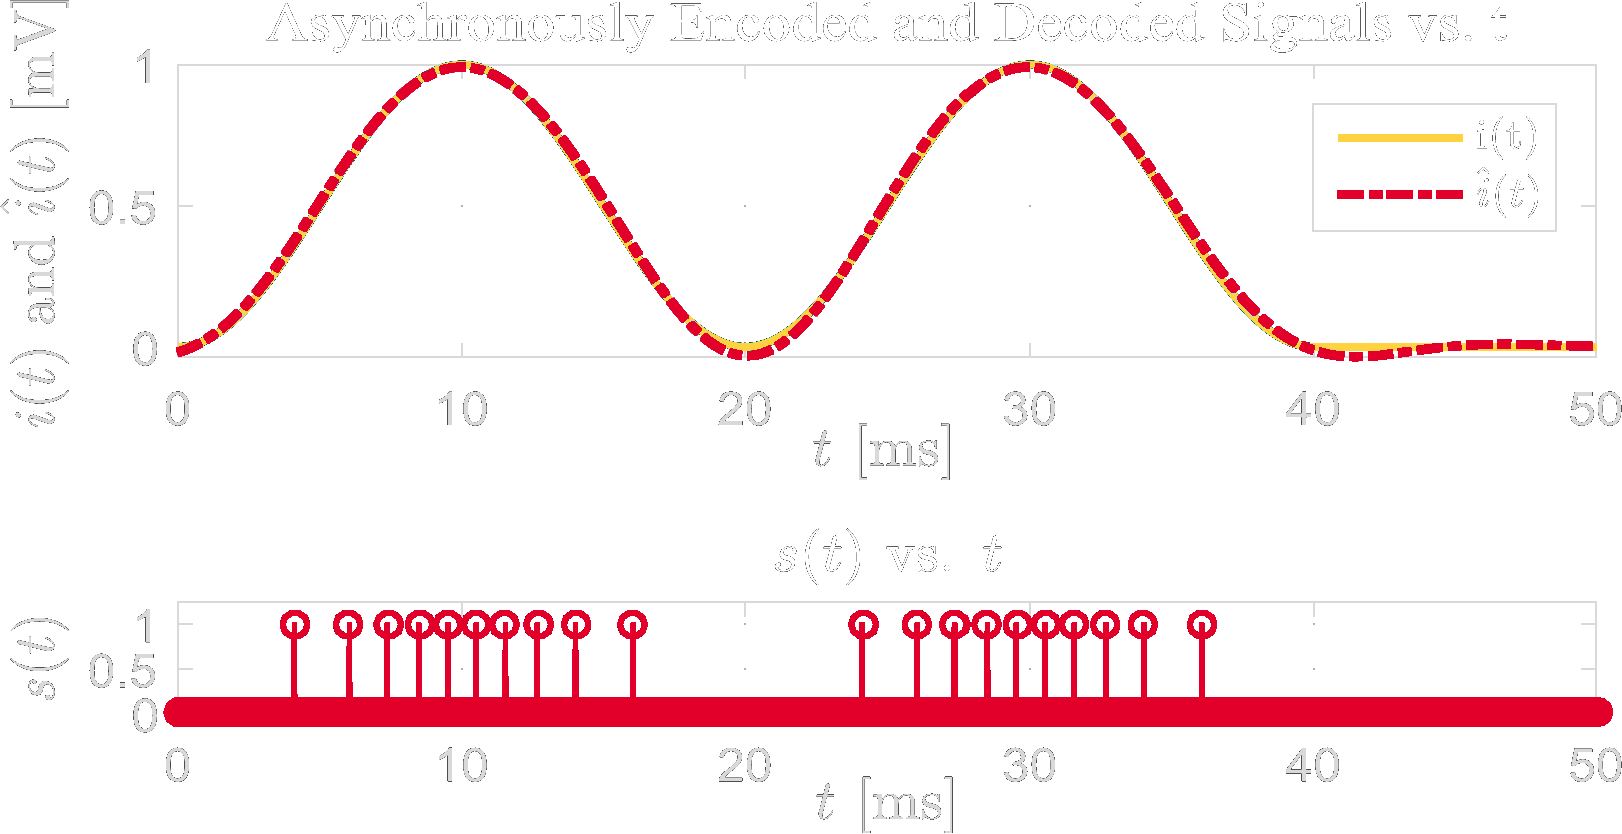
\includegraphics[scale=0.5]{Figures/signal_io.png}
    \end{figure}

    \column{0.45\paperwidth}
    \begin{figure}
        \centering
        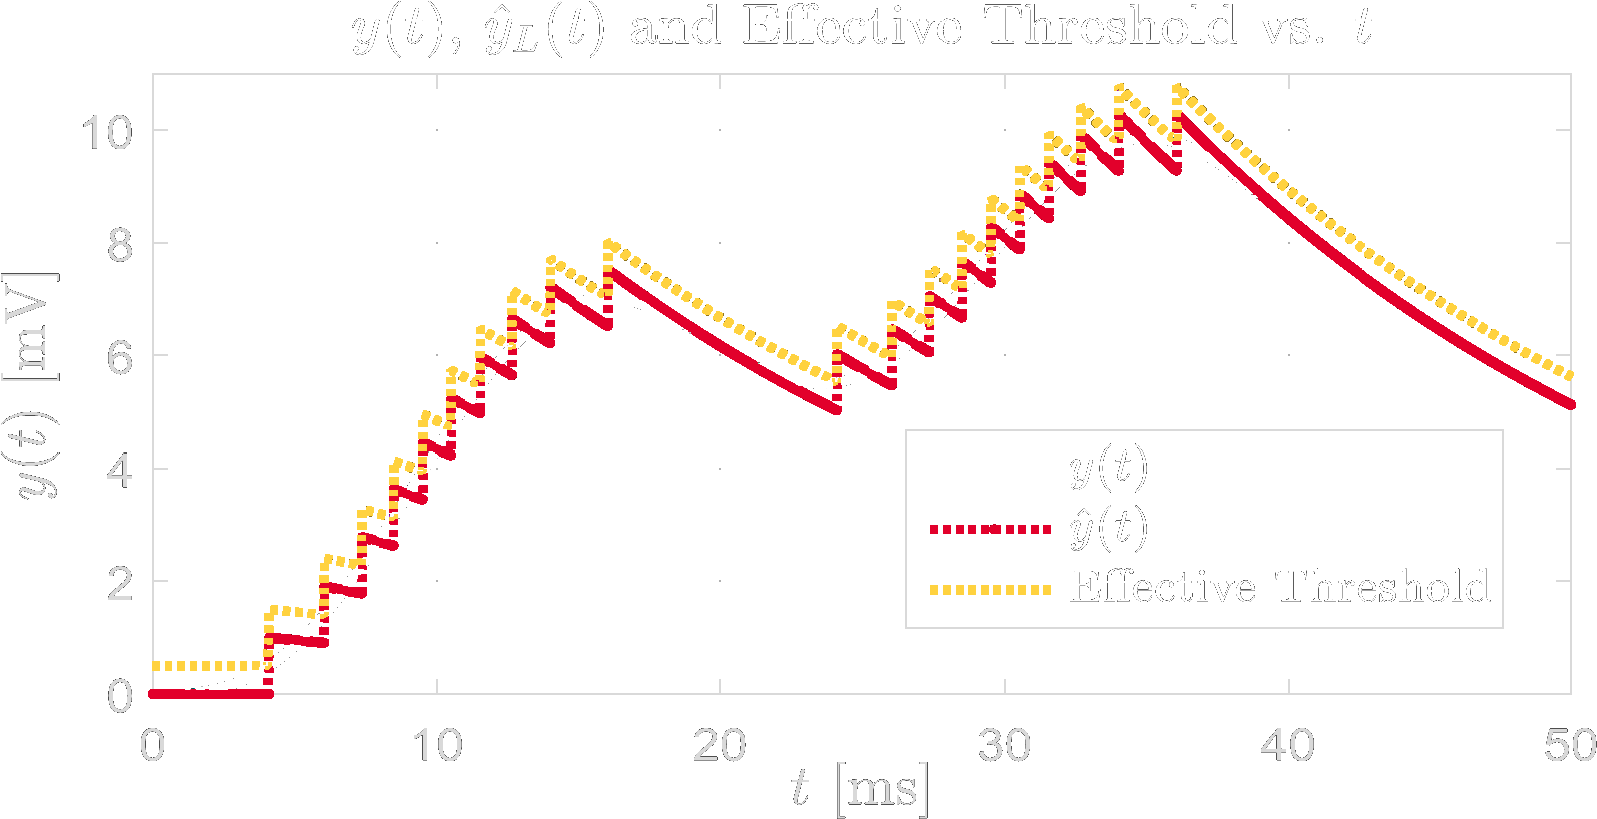
\includegraphics[scale=0.5]{Figures/signal_y.png}
    \end{figure}
    \begin{figure}
        \centering
        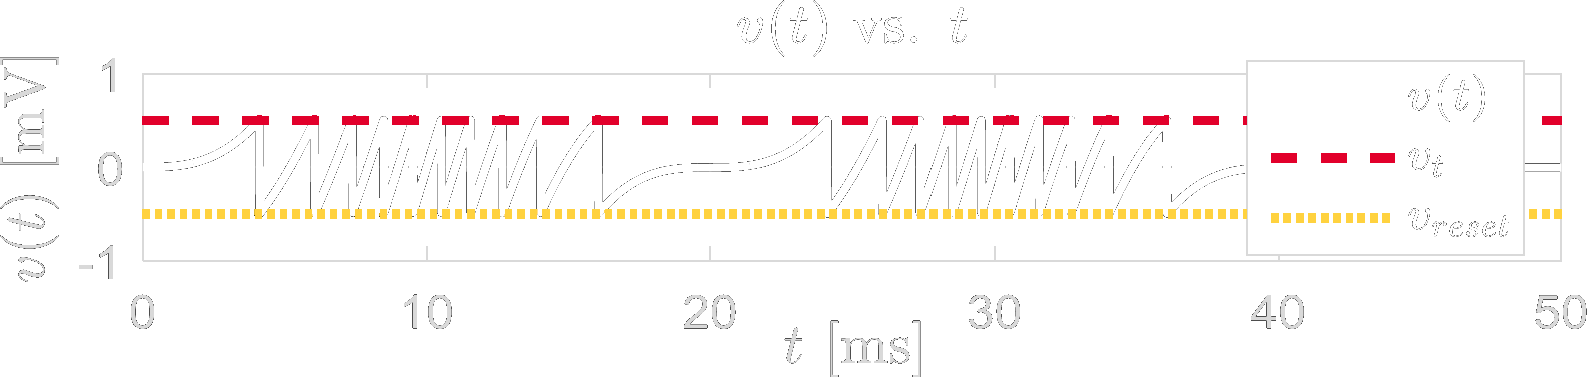
\includegraphics[scale=0.5]{Figures/signal_v.png}
    \end{figure}

    \end{columns}
\end{frame}


\section{Sigma-Delta Modulation}
\subsection{Canonical Form}
\begin{frame}{Where is the integral ?}{\insertsection ~- \insertsubsection}
    \begin{figure}
        \centering
        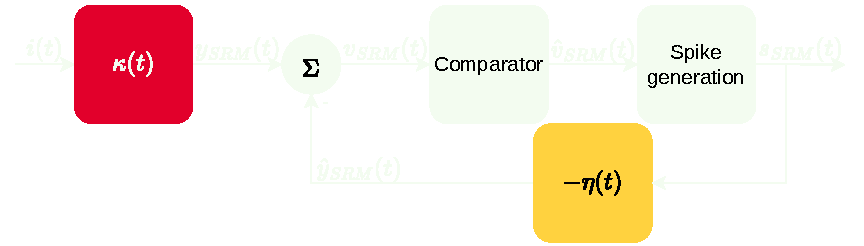
\includegraphics[width=.9\columnwidth]{Figures/srm_filter_simp.pdf}
    \end{figure}
\end{frame}

\begin{frame}{Special case}{\insertsection ~- \insertsubsection}
    \begin{columns}
    \column{0.4\paperwidth}
    \only<1->{
    \begin{figure}
        \centering
        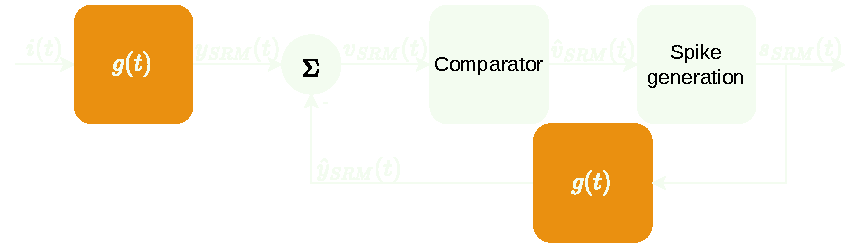
\includegraphics[width=\columnwidth]{Figures/srm_filter_spec.pdf}
    \end{figure}
    }
    \only<2->{
    \begin{figure}
        \centering
        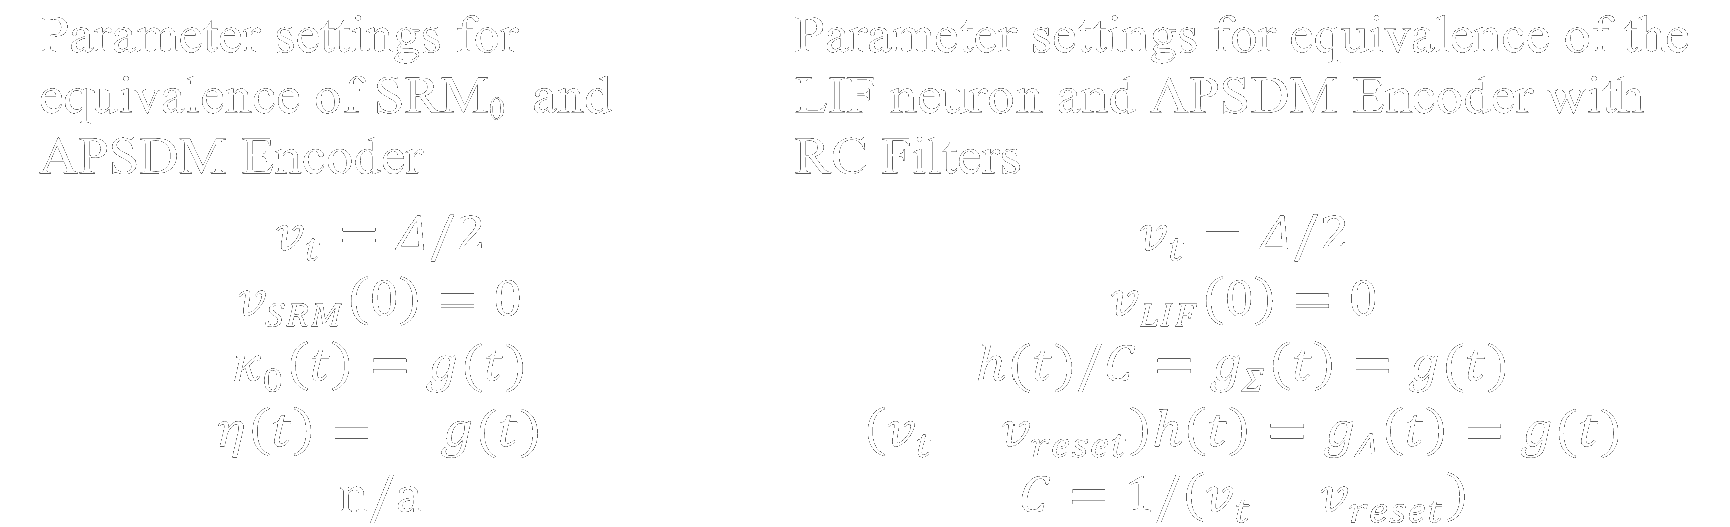
\includegraphics[width=\columnwidth]{Figures/condition.png}
    \end{figure}
    }


    \column{0.55\paperwidth}
    \only<2->{
    \begin{figure}
        \centering
        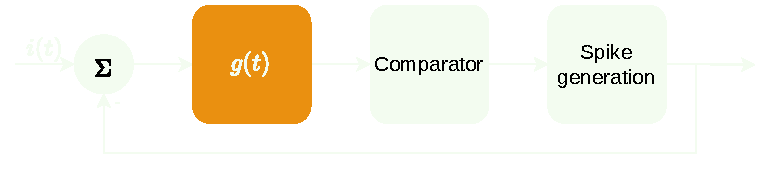
\includegraphics[width=\columnwidth]{Figures/srm_filter_spec_simp.pdf}
    \end{figure}
    }
    \only<3->{
    \begin{figure}
        \centering
        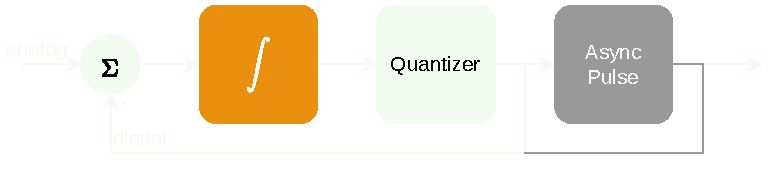
\includegraphics[width=\columnwidth]{Figures/sdm_canon.pdf}
    \end{figure}
    }

    \end{columns}
\end{frame}

\section{Demodulation}
\begin{frame}{\insertsection}

    \only<1>{
    \begin{figure}
        \centering
        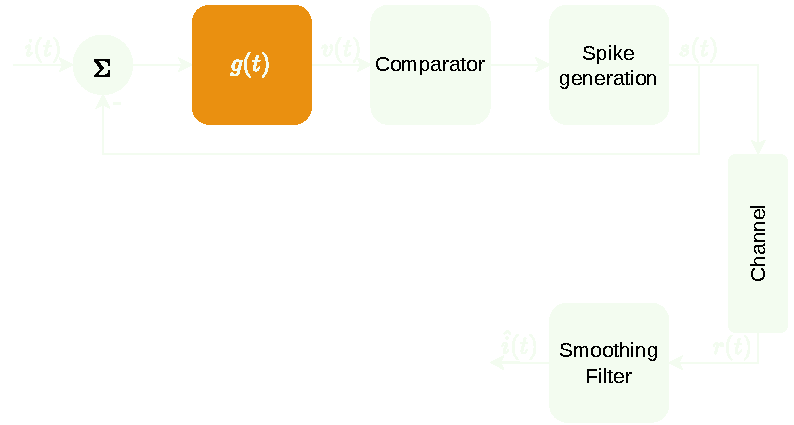
\includegraphics[width=.9\columnwidth]{Figures/sender_receiver.pdf}
    \end{figure}
    }
    \only<2>{
    \begin{figure}
        \centering
        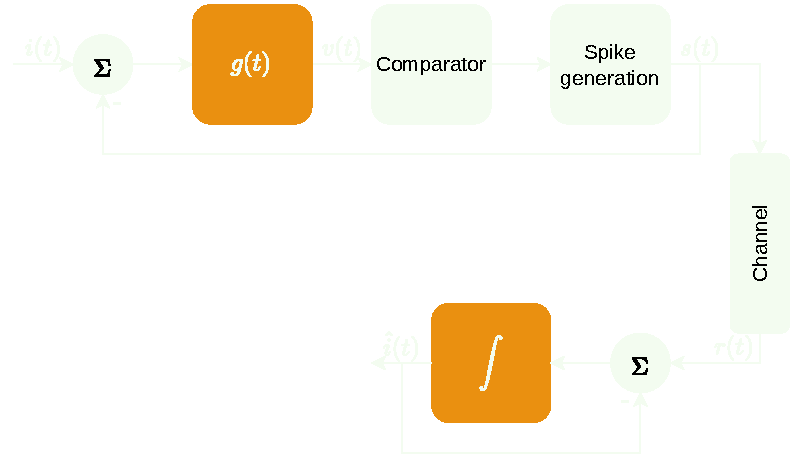
\includegraphics[width=.9\columnwidth]{Figures/sender_receiver_LI.pdf}
    \end{figure}
    }
\end{frame}

\section{Conclusion}
\begin{frame}{Summary}{\insertsection}
    \begin{figure}
        \centering
        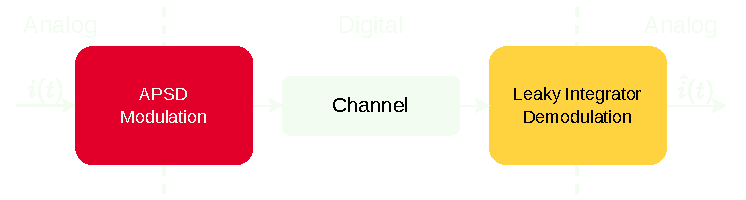
\includegraphics[width=.8\columnwidth]{Figures/overview.pdf}
    \end{figure}
    \begin{itemize}
        \item Formulation as the difference of an input response filter and its approximation
        \begin{itemize}
            \item Approximation error and spike frequency both depend on the threshold
        \end{itemize}
        \item Can be mapped to asynchronous pulse sigma-delta modulation
        \item Demodulation can be done by a low pass filter such as a Leaky Integrator
    \end{itemize}
\end{frame}

\begin{frame}{Perspectives}{\insertsection}
    \begin{itemize}
        \item APSDM is a simple case (unipolar, one threshold) but it can be extended (e.g. bipolar send-on-delta)
        \item What does it mean for processing with neurons ? \item How do we relate this with numerical solvers ?
        \item How can we exploit this structure to produce neuromorphic HW ?
        \item How biologically plausible is all of that ?
        \begin{itemize}
            \item Neuronal Spike Generation Mechanism as an Oversampling, Noise-shaping A-to-D Converter - Chklovskii & Soudry \cite{chklovskii_neuronal_2012}
        \end{itemize}
    \end{itemize}

    Further reading : \cite{schindler_linear_1974}, \cite{kikkert_asynchronous_1975}
\end{frame}

\appendix
\begingroup
  % \addtocounter{part}{-1}
    \part{Appendices}
    % \AtBeginSection[]{
    %     \begin{nonumberframe}{Table of contents}
    %         \tableofcontents[currentsection,part={2}]
    %     \end{nonumberframe}
    % }

    \section{References}
    \begin{frame}[allowframebreaks]{\insertsection}
      \printbibliography
    \end{frame}

    % \input{Parts/backup.tex}
\endgroup

\end{document}
